\chapter{网络连接}

\section{电话时代}

电话 (Telephone, 旧时音译作``德津风") 的线路是容易理解的, 早期的电话接线 (将通讯的两人连接起来) 要靠``接线生"人工操作.

电话线从用户家中通往电话局, 需要通电话时, 便拿起话筒说: ``接线生, 请给我接某某\dots\dots"

我们可以说, 这是一个以电话局为核心, 四面八方辐射向用户的\textbf{电话网络}.

使用这个网络进行通信时有三个要素: 呼叫的用户, 电话局的接线员, 被叫的用户. 往后我们可以看到, 不管是什么网络, 总是不可或缺这三个要素.

在以前, 电话只有一些企事业单位有, 要打电话的话就需要拨给对方工作的单位或家住处附近, 然后由人转接 (或者把人叫过来接电话), 于是又衍生出了传呼服务和查号台. 当年的查号台是 114, 由于查号台和DNS的功能很像, 所以 \verb|114.114.114.114| 这个IP地址被富有商业头脑的人租下了\footnote{对于商业用途来说, IP地址只有租凭, 没有购买一说, 但实质上租期超过百年也差不多就是购买了.}.

\section{有线连接}

自电话时代以来, 有线连接一直是最具代表性, 最具教学意义的网络连接方式.

对于用户来说, 家用电脑一般都自带有线网卡, 只需将网线插入网卡, 并连接到路由器即可开始上网. 那么, 电脑是怎么连接上网络的呢?

连接网络需要经过以下几个步骤, 也可以看作是分为以下几层:

\subsection{光纤入户}

互联网服务提供商 (Internet Service Provider, ISP)\footnote{在我国主要有中国联通、中国电信和中国移动 (新近增加的中国广电还没有自营的线路)} 铺设一条光纤通道直到您的住宅附近的一个光纤交换机, 然后从光纤交换机引出许多条线路, 其中一条直达您家中.

不过在部分地区仍在使用旧线路,例如电话线、同轴电缆 (电视线路) 等, 亦有复用原先的居民楼线路, 只将外部到居民楼的线路改为光纤的.

您可能会好奇, 光纤的一头是用户的家, 那么另一头究竟通往哪里?

答案是, 任何地方. 就像电话局直接也有线路互相连接形成网络一样, ISP直接也有互相连接的线路, 各个国家直接也有国际信道, 太平洋和大西洋海底都有铺设海底电缆 (或海底光缆), 此外还有通过空中电波建立联络的信道 (这就是抽象意义上的信道了, 我们会在无线连接一章中做进一步说明).

\subsection{调制调解}

\begin{figure}[htbp]
    \centering
    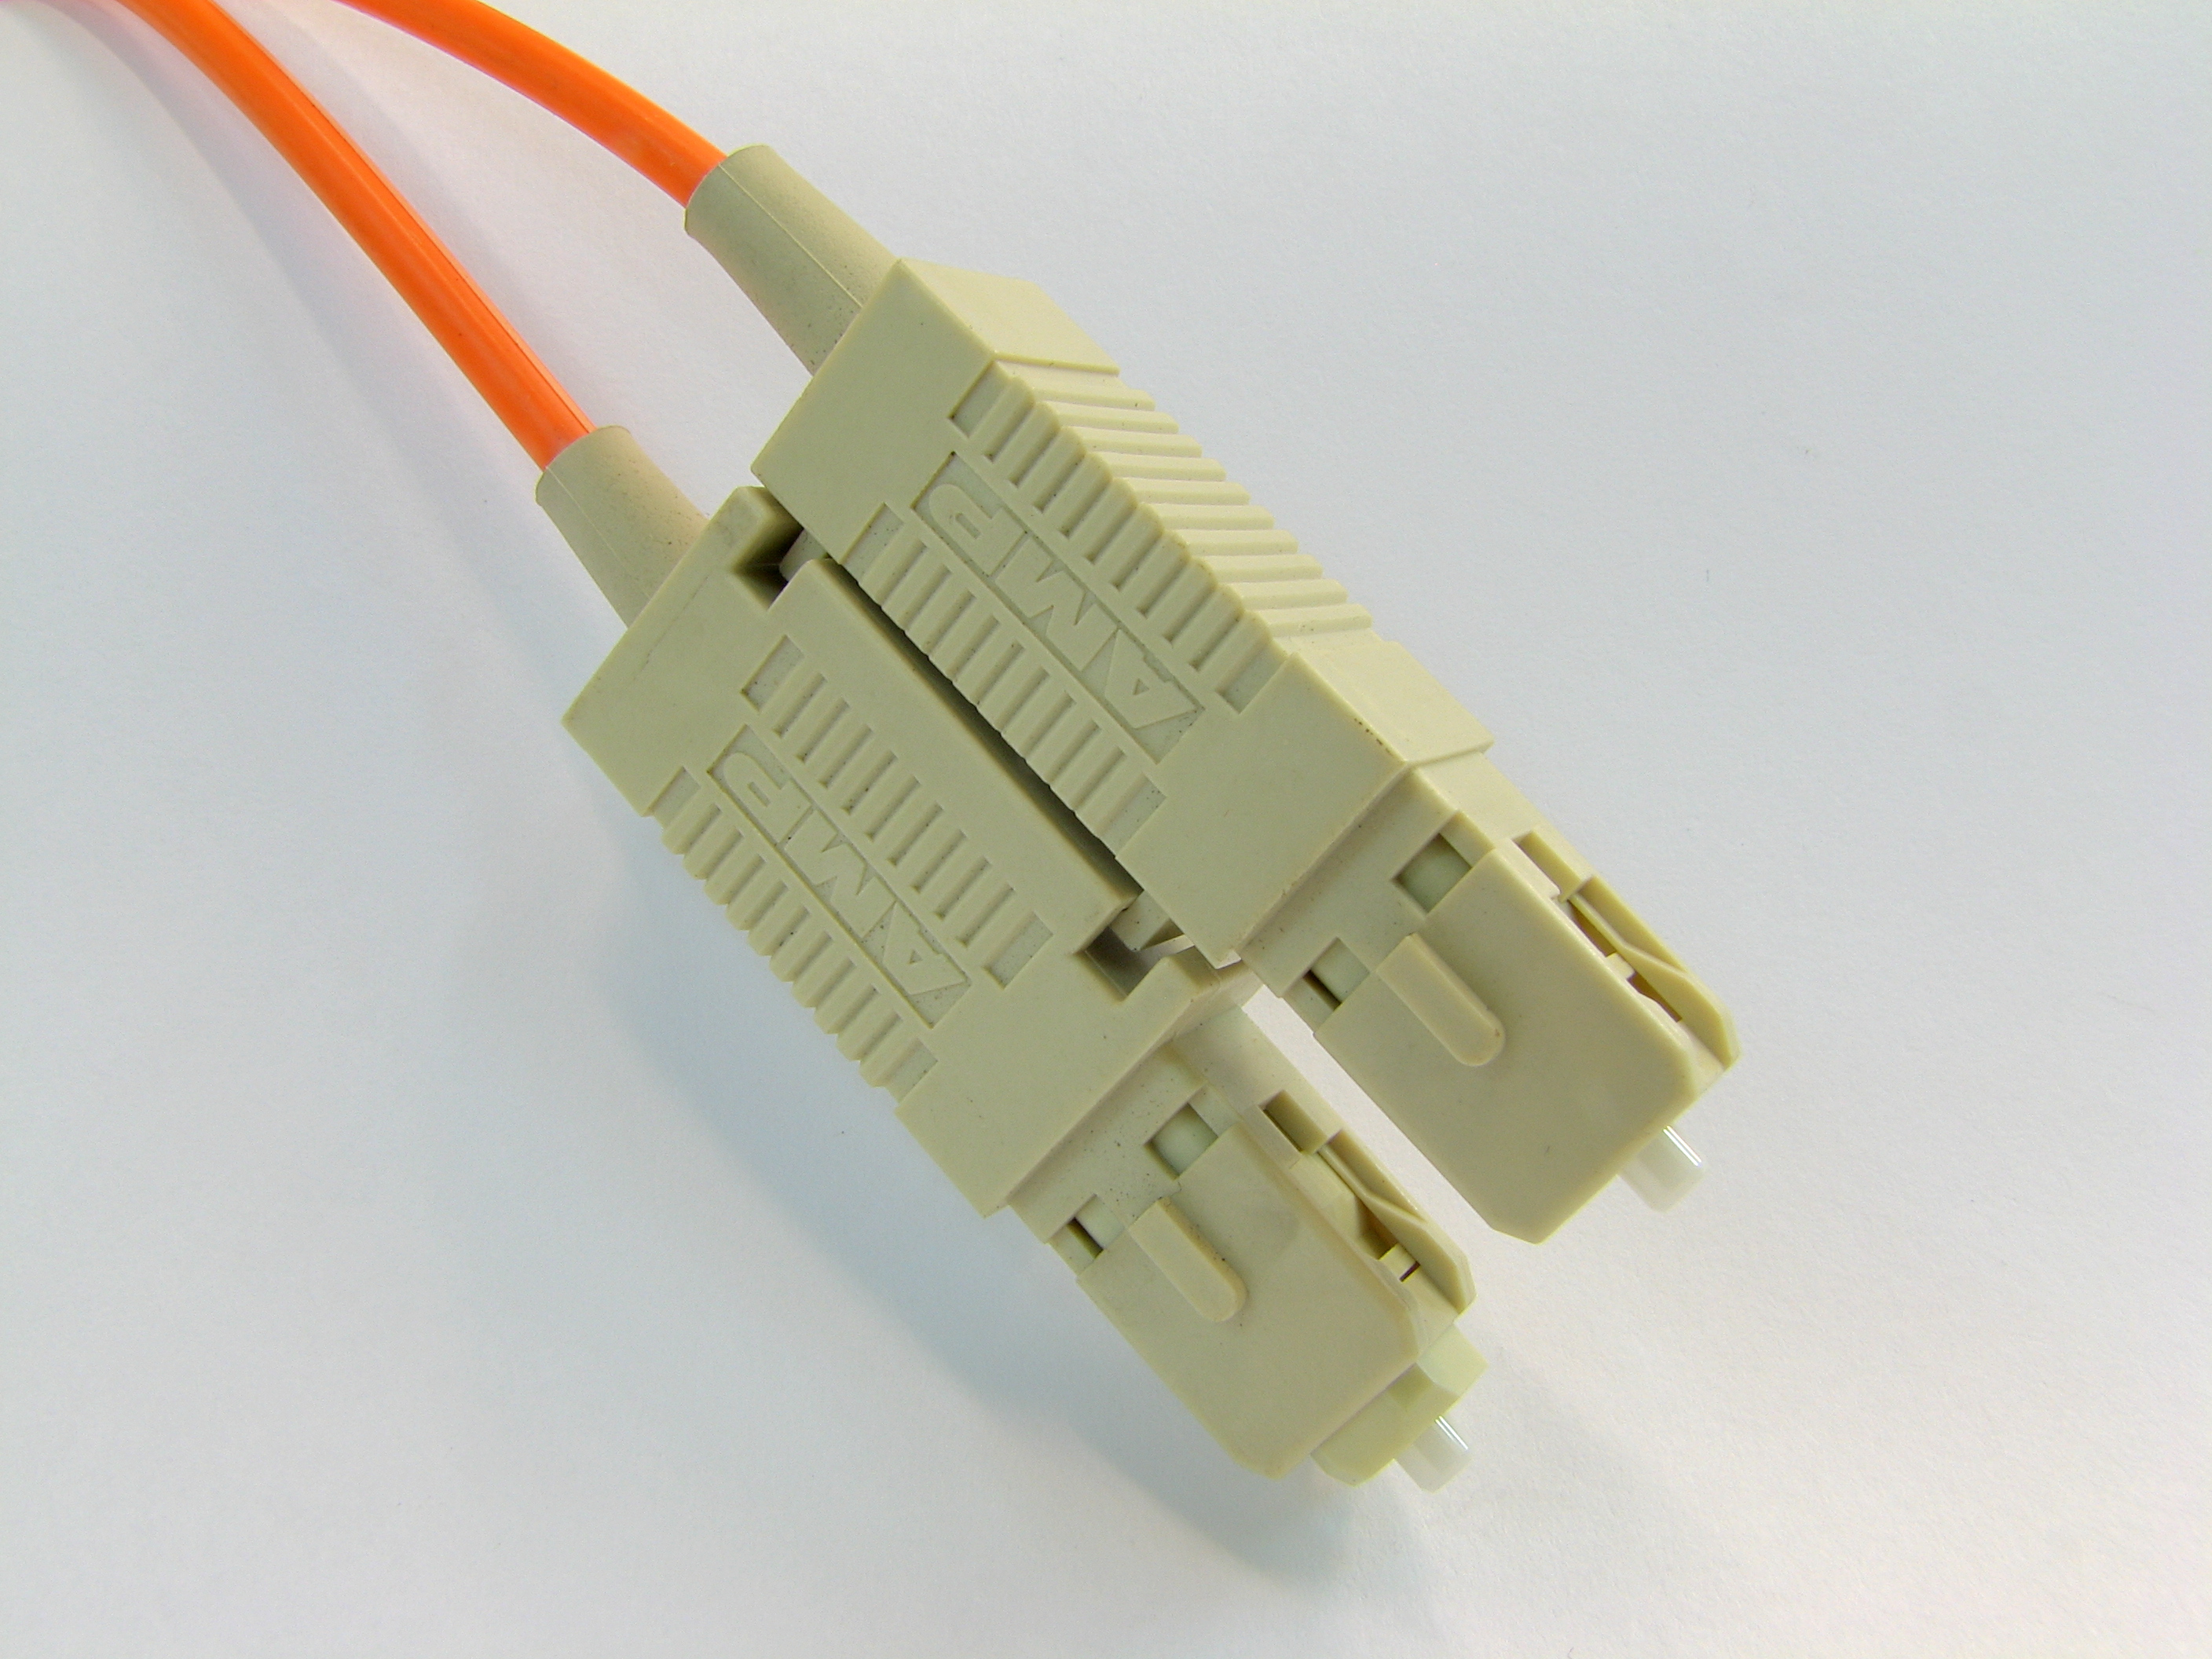
\includegraphics[width=2in]{media/SC-optical-fiber-connector-hdr-0a.jpg}
    \caption{入户光纤接线头
    \cite{OpticalFiberConnector}
    }
\end{figure}
\footfullcite{OpticalFiberConnector}

来自ISP的光纤进入您家中后不能直接用来上网, 从网线的\textit{RJ-45接口}和入户光纤接头不同这一点就很容易看出来. 更技术一些的理由是, 光纤使用的是光信号, 电脑的网线需要的是电信号, 必须要有一台设备将光信号和电信号互相转换才能连接网络.

ISP派来的员工为您上门安装宽带时通常会提供 (租给您) 一台\textit{调制调解器 (modulator-demodulator, 缩写 modem, 俗称``猫'')}, 这台设备可以将光信号与电信号相互转换, 并提供可用于电脑的网络接口.

有些Modem自带无线网络功能 (WLAN, 亦称Wi-Fi), \autoref*{sec:WLAN连接} 将会介绍这点.



\subsection{拨号}

这一过程经常由路由器完成, 常见的拨号协议为PPPoE(Point-to-Point Protocol over Ethernet, 以太网上的点对点协议).

以前用电话线上网的时候, 是由Modem (猫) 拨号到提供上网服务的号码, 常见的有 163 (这个数字也被富有商业头脑的人注册成为了域名, 一开始是提供邮箱服务的). 有一些电脑上配备了电话线接口, 可以省去Modem, 直接将电话线插到电脑上, 然后使用拨号上网软件就能连接网络.

电话拨号上网时的音频是人类不可读的, 只能听见哔啵声, 但是这段旋律成为了那个年代人们的回忆, 现在上网搜索可以找到相关录音.

\subsection{获取IP地址}

% TODO

\subsection{电脑连接路由器}

\begin{figure}[htbp]
    \centering
    \includesvg[width=2in]{media/Ethernet_plug_grey.svg}
    \caption{RJ-45线缆
    \cite{EthernetPlugGrey}
    }
\end{figure}
\footfullcite{EthernetPlugGrey}

\subsection{拨号}

% TODO

\section{WLAN连接}\label{sec:WLAN连接}

% TODO

\section{蜂窝网络}

% TODO

\endinput